\documentclass[11pt,largemargins]{homework}

\newcommand{\hwname}{Giulio Nenna}
\newcommand{\hwemail}{s245717@studenti.polito.it}
\newcommand{\hwtype}{Homework}
\newcommand{\hwnum}{2}
\newcommand{\hwclass}{}
\newcommand{\hwlecture}{}
\newcommand{\hwsection}{}

% This is just used to generate filler content. You don't need it in an actual
% homework!
\usepackage{lipsum}
\usepackage{amssymb}
\usepackage[utf8]{inputenc}
\usepackage[T1]{fontenc}
\usepackage{lmodern}
\usepackage{amsfonts}
\usepackage{hyperref}
\usepackage{bbm}
\usepackage{amsmath}
\usepackage{mcode}
\usepackage{epstopdf}
\usepackage{subcaption}
\usepackage{tikzit}
\input{Stilegrafo.tikzstyles}

\begin{document}
\maketitle
\begin{center}
Realizzato in collaborazione con Alfredo Baione (s279328)
\end{center}
\section{}% --------------ESERCIZIO 1------------------------------
  %\begin{figure}[htb]\centering
    %\includegraphics[scale=0.50]{grafoex1.jpg}
  %\end{figure}
  
    \ctikzfig{GrafoEx1}
    
  \begin{enumerate}
 
  
    \item
     Il numero di $1$ in $X(t)$ è:
     \begin{equation*}
     \eta\left(x\right)= \sum_{i=0}^{n}x_{i}.
     \end{equation*}
    Sia 
    \begin{equation*}
    N\left(t\right)=\eta\left(X\left(t\right)\right)=\sum_{i=1}^{n}X_{i}\left(t\right)
    \end{equation*}
     il numero dei nodi foglia infetti al tempo $t$.\\
     La matrice del kernel di mutazione riferita a tale processo è:
    \begin{equation*}
      \psi=
      \begin{bmatrix}
        1 & 0  \\
        1 & 0  \\
      \end{bmatrix},
      \end{equation*}
  mentre quelle associate al kernel di interazione sono:
   \begin{align*}
      \varphi\left(0\right)=\begin{bmatrix}
        1 & 0\\
        0 & 1 \\ 
      \end{bmatrix}, &&  
      \varphi\left(1\right)=\begin{bmatrix}
         0 & 1\\
        0 & 1 \\ 
      \end{bmatrix}.
    \end{align*}
    
     \`E possibile  osservare, allora, che le \emph{active boundaries} di $X(t)$ coincidono e sono solo solo funzioni di $\eta\left(x\right)$:
     \begin{equation*}
     \zeta_{01}\left(x\right)=\sum_{i,j}W_{ij}\left(1-x_{i}\right)x_{j}=\zeta_{10}\left(x\right)=\sum_{i,j}W_{ij}\left(1-x_{j}\right)x_{i}=n+1-\eta\left(x\right).
\end{equation*}     
 Ne risulta che $N\left(t\right)$ è una ``birth-and-death'' chain.\\
 Ponendo $N\left(t\right)=k$, risulta:
 \begin{align*}
 &\lambda_{N\left(t\right)}\left(x\right)=\left(n-k\right)\psi_{01}+\zeta_{01}\left(x\right)\beta\varphi_{01}\left(1\right)=\left(n-k\right)\cdot0+\left(n+1-\eta\left(x\right)\right)\cdot\beta=\left(n-k\right)\cdot\beta,\\
&\mu_{N\left(t\right)}\left(x\right)=k\psi_{10}+\zeta_{10}\left(x\right)\beta\varphi_{10}\left(0\right)=k+\left(n+1-\eta\left(x\right)\right)\cdot\beta\cdot0=k.\\
 \end{align*}
 
 
 \item
 Sia  $N\left(t\right)=k$. Nella costruzione dei rate di transizione della catena di Markov di nascita e morte $N\left(t\right)$, si ottiene: 
\begin{itemize}
\item
$\forall k < n$, \, \, $\lambda_{N\left(t\right)}\left(x\right)=\left(n-k\right)\cdot\beta>0$ \, \, $\left(k=1,...,n-1\right);$
\item
$\forall k >0$, \, \,  $\mu_{N\left(t\right)}\left(x\right)=k>0$ \, \, $\left(k=n,...,1\right).$
\end{itemize}
Pertanto, la catena è irriducibile.\\
L'unica distribuzione di probabilità invariante $\bar{\pi}$ di $N\left(t\right)$ avrà come componenti:
\begin{align*}
\bar{\pi}_{i}=\frac{1}{\sum_{k=0}^{n}\prod_{j=0}^{k-1}\frac{\lambda_{j}}{\mu_{j+1}}}\cdot\prod_{j=0}^{i-1}\frac{\lambda_{j}}{\mu_{j+1}}=\\
\frac{1}{\sum_{k=0}^{n}\prod_{j=0}^{k-1}\frac{\left(n-j\right)\cdot\beta}{j+1}}\cdot\prod_{j=0}^{i-1}\frac{\left(n-j\right)\cdot\beta}{j+1},&&i=0,...,n.
\end{align*}


\item
Sia $n=3$. Applicando la formula precedente, risulta che
\begin{align*}
\bar{\pi}_{i}=\frac{1}{\sum_{k=0}^{3}\prod_{j=0}^{k-1}\frac{\left(3-j\right)\cdot\beta}{j+1}}\cdot\prod_{j=0}^{i-1}\frac{\left(3-j\right)\cdot\beta}{j+1},&&i=0,...,3,
\end{align*}
da cui si ottiene:
\begin{align*}
\bar{\pi}_{0}=\frac{1}{1+3\beta+3\beta^{2}+\beta^{3}},\\
\bar{\pi}_{1}=\frac{3\beta}{1+3\beta+3\beta^{2}+\beta^{3}},\\
\bar{\pi}_{2}=\frac{3\beta^{2}}{1+3\beta+3\beta^{2}+\beta^{3}},\\
\bar{\pi}_{3}=\frac{\beta^{3}}{1+3\beta+3\beta^{2}+\beta^{3}}.
  \end{align*}
  Per capire quando $\bar{\pi}_{k}$, $k=0,...,3$, è massima, è possibile studiare il comportamento di $\bar{\pi}_{0}$, $\bar{\pi}_{1}$, $\bar{\pi}_{2}$ e $\bar{\pi}_{3}$, rispetto alla variabile $\beta$, nell'intervallo $[0,+\infty)$.
  
  %\begin{figure}[htb]\centering
%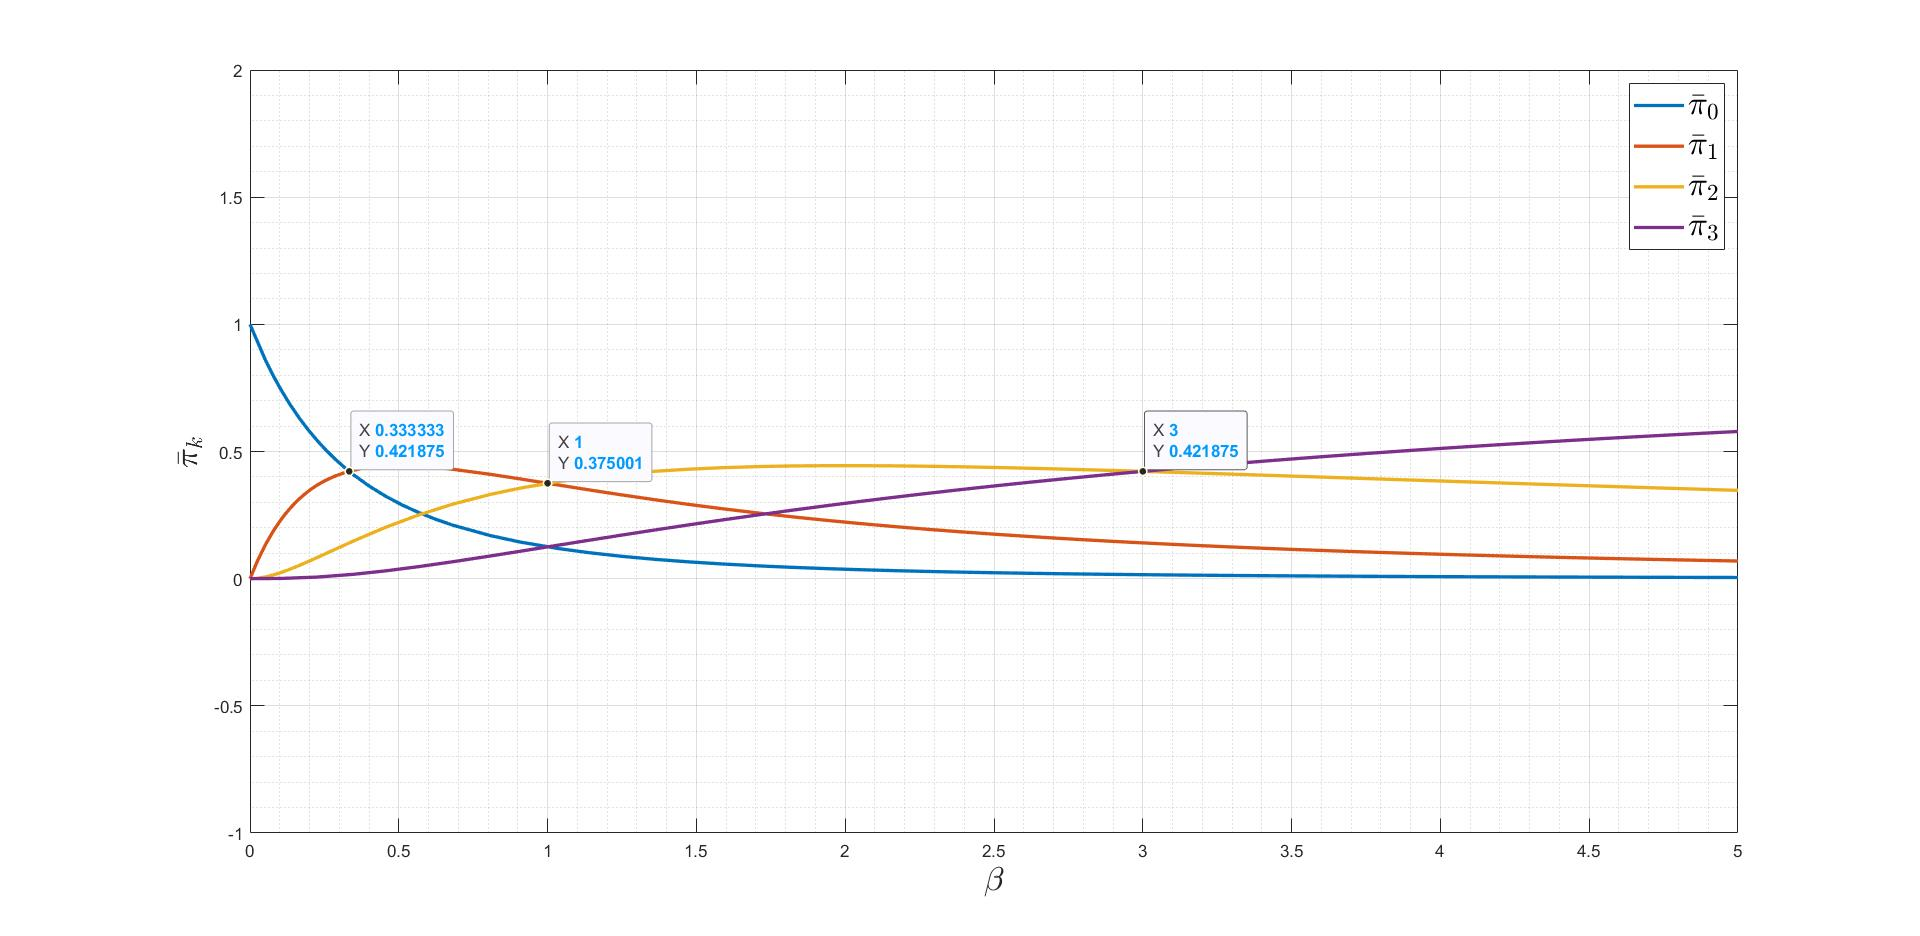
\includegraphics[scale=0.26]{ex1_3plot.jpg}
 % \end{figure}
  \newpage
  Come si evince dal grafico, allora:
  \begin{itemize}
  \item
  se  $0\leq\beta\leq\frac{1}{3}$,  $k=0$ è lo stato per cui $\bar{\pi}_{k}$ è massima;
  \item
  se  $\frac{1}{3}\leq\beta\leq 1$,  $k=1$ è lo stato per cui $\bar{\pi}_{k}$ è massima;
  \item
  se  $1\leq\beta\leq 3$,  $k=2$ è lo stato per cui $\bar{\pi}_{k}$ è massima;
  \item
  se  $3\leq\beta< +\infty$,  $k=3$ è lo stato per cui $\bar{\pi}_{k}$ è massima.
  \end{itemize}
 
  \item
  Sia 
  \begin{align*}  
  k_{n}= \underset{k=0,...,n}{\arg\max} \, \, (\bar{\pi}_{k}).
  \end{align*}
  La catena di disuguaglianze
  \begin{align*}
  \frac{\bar{\pi}_{i+1}}{\bar{\pi}_{i}} \geq 1\Leftrightarrow\frac{\lambda_{j}}{\mu_{j+1}}\geq 1\Leftrightarrow(n-j)\cdot\beta\geq j\Leftrightarrow\ n\beta-j\beta \geq j 
  \Leftrightarrow 
  j+j\beta \leq n\beta
 \Leftrightarrow j \leq \frac{n\beta}{1+\beta}
 \end{align*}
 prova che:
 \begin{align*}
k_{n}= \underset{k=0,...,n}{\arg\max} \, \, (\bar{\pi}_{k}) =\Bigl\lfloor\frac{n\beta}{1+\beta}\Bigr\rfloor=\frac{n\beta}{1+\beta}-\epsilon,&& 0\leq \epsilon<1.
 \end{align*} 
 Pertanto, si avrà:
  \begin{align*}
  \lim\limits_{n \rightarrow +\infty}\frac{k_{n}}{n}=\lim\limits_{n \rightarrow \infty}\left(\frac{n\beta}{n\left(1+\beta\right)}-\frac{\epsilon}{n}\right)=\frac{\beta}{1+\beta}.
  \end{align*}
  
    

  \end{enumerate}

  \newpage
\section{}%---------------ESERCIZIO 2-----------------------------------
 
%\begin{figure}[htb]\centering
%\includegraphics[scale=0.50]{grafoex2.png}
 % \end{figure}
  \ctikzfig{GrafoEx2}
 \begin{alphaparts}
    \questionpart

    Agli archi $\emph{e}_{1}$ ed $\emph{e}_{2}$ corrispondono le funzioni di costo 
    \begin{align*}
    \Delta_{1}=\omega_{1} && e && \Delta_{2}=\omega_{2}+\frac{3}{2}f_{2},
    \end{align*}
   dove $\omega_{1}$ e $\omega_{2}$ rappresentano i pedaggi applicati al passaggio dei corrispondenti flussi $\emph{f}_{1}$ e $\emph{f}_{2}$, tali che $\emph{f}_{1}+\emph{f}_{2}=1$.\\
    Risulta che $\emph{f}^{(\omega)}=\left(f_{1}^{(\omega)},f_{2}^{(\omega)}\right)$  è  ``equilibrio  di  Wardrop'' se e solo se:
    \begin{align*}    
    \begin{cases}f_{1}^{(\omega)}>0  \Rightarrow  \Delta_{1}\leq\Delta_{2}  \Leftrightarrow  \omega_{1}  \leq  \omega_{2}+\frac{3}{2}f_{2}^{(\omega)}\\
    f_{2}^{(\omega)}>0  \Rightarrow  \Delta_{2}\leq\Delta_{1}  \Leftrightarrow  \omega_{1}  \geq  \omega_{2}+\frac{3}{2}f_{2}^{(\omega)}\end{cases}
    \Leftrightarrow \begin{cases}f_{2}^{(\omega)}=\frac{2}{3}\left(\omega_{1}-\omega_{2}\right)\\ f_{1}^{(\omega)}=1-\frac{2}{3}\left(\omega_{1}-\omega_{2}\right).\end{cases}
    \end{align*}
    
    %---------------------------------------------------------------------------------
    \questionpart
    Si consideri il gioco
    \begin{equation*}
    \left(\mathcal{V}=\{1,2\}, \, A=\{0,1\},\, U=\{u_{i}\left(\omega_{1},\omega_{2}\right)=\omega_{i}f_{i}^{(\omega)}, \, i=1,2\}\right),
    \end{equation*}
    dove $1$ e $2$ rappresentano, rispettivamente, i gestori dei nodi $o$ e $d$ del suddetto grafo.\\
    La funzione di \emph{best response} del primo giocatore risulta essere
    \begin{gather*}
    BR_{1}\left(\omega_{2}\right)=\underset{\omega_{1}\in A}{\arg\max} \, \, u_{1}\left(\omega_{1},\omega_{2}\right)= \underset{\omega_{1}\in A}{\arg\max} \, \, \omega_{1}f_{1}^{(\omega)}=\\ 
    \underset{\omega_{1}\in A}{\arg\max} \, \, \omega_{1}\left(1-\frac{2}{3}\left(\omega_{1}-\omega_{2}\right)\right)=
 \underset{\omega_{1}\in A}{\arg\max} \, \, \omega_{1}\left(1-\frac{2}{3}\omega_{1}+\frac{2}{3}\omega_{2}\right)=\\ \underset{\omega_{1}\in A}{\arg\max} \, \, \left(\omega_{1}-\frac{2}{3}\omega_{1}^{2}+\frac{2}{3}\omega_{1}\omega_{2}\right)=\frac{3}{4}+\frac{1}{2}\omega_{2},  
    \end{gather*}
    mentre quella relativa al secondo é
    \begin{gather*}
     BR_{2}\left(\omega_{1}\right)=\underset{\omega_{2}\in A}{\arg\max} \, \, u_{2}\left(\omega_{2},\omega_{1}\right)= \underset{\omega_{2}\in A}{\arg\max} \, \, \omega_{2}f_{2}^{(\omega)}= \\
     \underset{\omega_{2}\in A}{\arg\max} \, \, \omega_{2}\left(\frac{2}{3}\left(\omega_{1}-\omega_{2}\right)\right)=
 \underset{\omega_{2}\in A}{\arg\max} \, \, \omega_{2}\left(\frac{2}{3}\omega_{1}-\frac{2}{3}\omega_{2}\right)=\\
 \underset{\omega_{2}\in A}{\arg\max} \, \, \left(\frac{2}{3}\omega_{2}\omega_{1}-\frac{2}{3}\omega_{2}^{2}\right)=\frac{1}{2}\omega_{1}.
    \end{gather*}
    

    %----------------------------------------------------------------------------------

    \questionpart
    Per trovare l'equilibrio di Nash del gioco in questione, si deve imporre che ogni giocatore giochi la sua \emph{best response}, in risposta all'azione dell'altro giocatore. In tal caso, questo si traduce nella risoluzione del seguente sistema:
    \begin{equation*}
    \begin{cases}\omega_{1}^{*}=\frac{3}{4}+\frac{1}{2}\omega_{2}^{*}\\
    \omega_{2}^{*}=\frac{1}{2}\omega_{1}^{*}\end{cases}\Leftrightarrow
    \begin{cases}\omega_{1}^{*}=\frac{3}{4}+\frac{1}{2}\left(\frac{1}{2}\omega_{1}^{*}\right)\\
    \omega_{2}^{*}=\frac{1}{2}\omega_{1}^{*}\end{cases}\Leftrightarrow\begin{cases}\omega_{1}^{*}=1\\\omega_{2}^{*}=\frac{1}{2}\end{cases},
    \end{equation*}
    e tali sono i valori degli equilibri di Nash cercati.
    \end{alphaparts}
    
    
\newpage

\section{}%---------------ESERCIZIO 3 ------------------------------------------

Si consideri il gioco $\left(\mathcal{V},A,\{u_{i}\}\right),$ caratterizzato da
\begin{align*}
\mathcal{V}=\{1,2,...,n\}, && A=\{-1,+1\}, && u_{i}\left(x_{i},x_{-i}\right)=\begin{cases}\frac{1}{2}\sum_{j\neq i}\mid x_{i}+x_{j}\mid \,\, se \, \, i\in \mathcal{V}_{1}\\\frac{1}{2}\sum_{j\neq i}\mid x_{i}-x_{j}\mid \,\, se \, \, i\in \mathcal{V}_{2}\end{cases},
\end{align*}
dove
\begin{align*}
\mathcal{V}_{1}=\{1,2,...,n_{1}\} \, \, \, \text{e} \, \, \, \mathcal{V}_{2}=\{n_{1}+1,n_{1}+2,...,n\}.
\end{align*}

\begin{alphaparts}
\questionpart
Sia $n=3$.


  
  \begin{itemize}
  
  
    \item[$\left(\textbf{a1}\right)$]  $n_{1}=3$.\\
  Ciascun giocatore sta giocando un coordination game quindi valgono le seguenti: 
  \begin{align*}
  \mathcal{V}_{1}=\{1,2,3\}, \, \mathcal{V}_{2}=\emptyset, \\
   u_{i}=\frac{1}{2}\sum_{j\neq i}\mid x_{i}+x_{j}\mid, \,\, \forall i.
  \end{align*}
  Se definiamo le quantità
  \begin{gather*}
    n^+ = | \{x_i = +1, i\in \mathcal{V}\}|\\
    n^- = | \{x_i = -1, i\in \mathcal{V}\}|
  \end{gather*}
  che rappresentano rispettivamente il numero di giocatori che stanno giocando +1 e -1 allora per ciascun giocatore vale la seguente:
  \begin{gather*}
    \{x_i = +1\} \in BR_i (x_{-i}) \iff n^+ \geq n^-\\
    \{x_i = -1\} \in BR_i (x_{-i}) \iff n^- \geq n^+
  \end{gather*}
  
  Gli equilibri di Nash, pertanto, saranno dati dalle terne $\left(-1,-1,-1\right)$ e $\left(+1,+1,+1\right)$, perché entrambe le configurazioni, in tal caso, massimizzano le ``utilities'' di $1$, $2$ e $3$ e sono compatibili con i best response di ciascun giocatore.
  
  
  \item[$\left(\textbf{a2}\right)$] $n_{1}=2$.\\%----------------------------------------------------------------------------
  In questo caso il giocatore \(i = 3\) sta giocando un anti-coordination game. Quindi: 
  \begin{gather*}
  \mathcal{V}_{1}=\{1,2\}, \, \mathcal{V}_{2}=\{3\},\\
  u_{1}=\frac{1}{2}\cdot \left(\mid x_{1}+x_{2}\mid + \mid x_{1}+x_{3}\mid\right), \\ u_{2}=\frac{1}{2}\cdot \left(\mid x_{2}+x_{1}\mid + \mid x_{2}+x_{3}\mid\right), \\ u_{3}=\frac{1}{2}\cdot \left(\mid x_{3}-x_{1}\mid + \mid x_{3}-x_{2}\mid\right).
  \end{gather*}
  Per cui vale:
  \begin{gather*}
    \{x_3 = +1\} \in BR_3 (x_{-3}) \iff n^- \geq n^+\\
    \{x_3 = -1\} \in BR_3 (x_{-3}) \iff n^+ \geq n^-
  \end{gather*}


  Quindi, gli equilibri di Nash risultano essere individuati dalle configurazioni $\left(-1,-1,+1\right)$ e $\left(+1,+1,-1\right)$ in cui si può notare come ai primi due giocatori convenga essere "accordati" mentre al terzo convenga giocare il contrario di quello che giocano i primi due.
  
  
  \item[$\left(\textbf{a3}\right)$]  $n_{1}=1$.\\ %-------------------------------------------------------------------------
  In questo caso due dei tre giocatori sta giocando un anti-coordination game e solo il terzo sta giocando un coordination game. In particolare:
  \begin{gather*}
  \mathcal{V}_{1}=\{1\},\, \mathcal{V}_{2}=\{2,3\},\\
  u_{1}=\frac{1}{2}\cdot \left(\mid x_{1}+x_{2}\mid + \mid x_{1}+x_{3}\mid\right), \\
  u_{2}=\frac{1}{2}\cdot \left(\mid x_{2}-x_{1}\mid + \mid x_{2}-x_{3}\mid\right), \\
  u_{3}=\frac{1}{2}\cdot \left(\mid x_{3}-x_{1}\mid + \mid x_{3}-x_{2}\mid\right).
  \end{gather*}
  
  Gli equilibri di Nash sono individuati da $\left(+1,+1,-1\right)$, $\left(-1,+1,-1\right)$, $\left(+1,-1,+1\right)$ e $\left(-1,-1,+1\right)$, ossia configurazioni in cui fintanto che \(x_1 \neq x_2\) allora \(i=1\) può giocare qualsiasi valore dal momento che la sua utilità non cambia. In queste configurazioni nessun giocatore guadagna utilità cambiando mossa.
  
  
  
  \item[$\left(\textbf{a4}\right)$] $n_{1}=0$.\\%--------------------------------------------------------------------------
  Tutti i giocatori stanno giocando un anti-coordination game:
  \begin{align*}
  \mathcal{V}_{1}=\emptyset, \, \mathcal{V}_{2}=\{1,2,3\},\\
  u_{i}=\frac{1}{2}\sum_{j\neq i}\mid x_{i}-x_{j}\mid, \,\, \forall i
  \end{align*}
  e gli stati $\left(+1,-1,-1\right)$, $\left(-1,+1,-1\right)$, $\left(-1,-1,+1\right)$, $\left(-1,+1,+1\right)$, $\left(+1,-1,+1\right)$ e $\left(+1,+1,-1\right)$ saranno equilibri di Nash, per le ragioni già esposte. Queste configurazioni rappresentano tutte le possibili combinazioni di mosse dei giocatori tranne quelle in cui sono tutti accordati, incompatibili con i best response di qualsiasi giocatore nel caso di un anti-coordination game.
  \end{itemize}
  
  
  
  \newpage
  \questionpart
  Sia $n=3$ e $X\left(0\right)=\left(+1,-1,+1\right)$ la configurazione iniziale della catena di Markov $X\left(t\right)$, a tempo continuo, corrispondente alla dinamica di \emph{best response} asincrona per il gioco di sopra. \\
  \begin{itemize}
  
 \item[$\left(\textbf{b1}\right)$] $n_{1}=3$. 
 
 \ctikzfig{Grafo1}
 
 Per questo punto e per quelli successivi verrà utilizzata la nomenclatura mostrata in figura. In particolare \(x_i\) rappresenta la i-esima configurazione nel grafo delle transizioni e gli archi sono colorati in rosso, blu o verde se a cambiare mossa in un salto di configurazione sono rispettivamente il primo, il secondo o il terzo giocatore.  \\

  Come si può osservare dal grafo delle transizioni di configurazione con i relativi \emph{rate} di transizione, risulta che
  \begin{equation*}
  \lim\limits_{t \rightarrow +\infty}\mathbb{P}\left(X\left(t\right)=x\mid X\left(0\right)=\left(+1,-1,+1\right)\right)=\left(\frac{1}{2},\frac{1}{2},0,0,0,0,0,0\right)',
\end{equation*}
in quanto $X\left(t\right)$, per $t\mapsto +\infty$, finirà necessariamente in uno dei due stati assorbenti, $\left(-1,-1,-1\right)$ oppure $\left(+1,+1,+1\right)$, con probabilità pari a $\frac{1}{2}$ per entrambi.

\newpage
   \item[$\left(\textbf{b2}\right)$] $n_{1}=2$. 
 
   \ctikzfig{Grafo2}
 
   %\begin{figure}[htb]\centering
%\includegraphics[scale=0.50]{transitiongraph2.png}
  %\end{figure}  
  
  Il grafo di transizione, in tal caso, è fortemente connesso. Questo significa che esiste una sola misura invariante, $\pi_{x}$, a cui tenderà $$\lim\limits_{t \rightarrow +\infty}\mathbb{P}\left(X\left(t\right)=x\mid X\left(0\right)=\left(+1,-1,+1\right)\right).$$
  Sfruttando allora l'esistenza di 4 simmetrie, identificabili con $\pi_{a}$, $\pi_{b}$, $\pi_{c}$ e $\pi_{d}$ (ognuna associata ad un raggruppamento di colore diverso in figura) è possibile determinare la misura invariante \(\pi_x\) traducendo la condizione 
  \begin{gather*}
    L'\pi = 0 \iff \text{diag}(\omega)\pi = \Lambda ' \pi
  \end{gather*}
  in
  \begin{equation*}
  \begin{cases}
    \pi_{a}=\pi_{c}+\pi_{b}\\
    2\pi_{b}=\frac{1}{2}\pi_c+ \frac{1}{2}\pi_d\\
    2\pi_{c}=\frac{1}{2}\pi_{b}+\frac{1}{2}\pi_{d}\\
    \pi_{a}+\pi_{b}+\pi_{c}+\pi_{d}=\frac{1}{2}
  \end{cases}
  \Leftrightarrow
  \begin{cases}
    \pi_{a}=\frac{2}{14}\\
    \pi_{b}=\frac{1}{14}\\
    \pi_{c}=\frac{1}{14}\\
    \pi_{d}=\frac{3}{14}
  \end{cases},
  \end{equation*}
  da cui si ricava che
  \begin{gather*}
  \lim\limits_{t \rightarrow +\infty}\mathbb{P}\left(X\left(t\right)=x\mid X\left(0\right)=\left(+1,-1,+1\right)\right)=\\
  =\pi_{x}=\frac{1}{14}\left(2, 2, 1, 1, 1, 1, 3, 3\right)'.
  \end{gather*}
  
  
  \newpage
   \item[$\left(\textbf{b3}\right)$] $n_{1}=1$. 
 %\begin{figure}[htb]\centering
%\includegraphics[scale=0.50]{transitiongraph3.png}
  %\end{figure} 
  \ctikzfig{Grafo3}
  Anche in tal caso il grafo di transizione risulta fortemente connesso e, quindi, esiste un'unica misura invariante, $\pi_{x}$, a cui tende $$\lim\limits_{t \rightarrow +\infty}\mathbb{P}\left(X\left(t\right)=x\mid X\left(0\right)=\left(+1,-1,+1\right)\right).$$\\
  Come prima, grazie  ai \emph{rates} di transizione tra i diversi stati e alle quattro simmetrie presenti nel grafo ($\pi_{a}$, $\pi_{b}$, $\pi_{c}$ e $\pi_{d}$), ricaviamo il sistema
  \begin{equation*}
  \begin{cases}
    2\pi_{a}=\pi_{b}\\
    \pi_{c}=\pi_{a}+\frac{1}{2}\pi_{b}+\frac{1}{2}\pi_{d}\\
    2\pi_{b}=\frac{1}{2}\pi_{c}+\frac{1}{2}\pi_{d}\\
    \pi_{a}+\pi_{b}+\pi_{c}+\pi_{d}=\frac{1}{2}
  \end{cases}
  \Leftrightarrow
  \begin{cases}\pi_{a}=\frac{1}{22}\\
  \pi_{c}=\pi_{d}=\frac{2}{11}\\
  \pi_{b}=\frac{1}{11}\end{cases},
  \end{equation*}
  da cui
  \begin{gather*}
  \lim\limits_{t \rightarrow +\infty}\mathbb{P}\left(X\left(t\right)=x\mid X\left(0\right)=\left(+1,-1,+1\right)\right)=\\
  =\pi_{x}=\left(\frac{1}{22},\frac{1}{22},\frac{1}{11},\frac{1}{11},\frac{2}{11},\frac{2}{11},\frac{2}{11},\frac{2}{11}\right)'.
  \end{gather*}
  
  \newpage
  \item[$\left(\textbf{b4}\right)$] $n_{1}=0$. 
 %\begin{figure}[htb]\centering
%\includegraphics[scale=0.50]{transitiongraph4.png}
  %\end{figure}
  
  
  \ctikzfig{Grafo4}
  In quest'ultima configurazione del grafo di transizione esiste un solo stato assorbente del sistema, per $t\mapsto +\infty$, rappresentato dall'insieme $\{x_{3}, \, x_{4}, \, x_{5}, \, x_{6}, \, x_{7}, \, x_{8}\}$.\\
  Pertanto, si avrà, analogamente al caso in cui \(n_1 = 3\):
  \begin{equation*}
  \lim\limits_{t \rightarrow +\infty}\mathbb{P}\left(X\left(t\right)=x\mid X\left(0\right)=\left(+1,-1,+1\right)\right)=\left(0,0,\frac{1}{6},\frac{1}{6},\frac{1}{6},\frac{1}{6},\frac{1}{6},\frac{1}{6}\right)'.
\end{equation*}
   
   \end{itemize}
   \end{alphaparts}
% Sometimes questions get separated from their bodies. Use a \newpage to force
% them to wrap to the next page.
% Use \renewcommand{\questiontype}{<text>} to change what word is displayed
% before numbered questions
%\renewcommand{\questiontype}{Task}
\end{document}
